\documentclass{article}

\usepackage{arxiv}

\usepackage[utf8]{inputenc} % allow utf-8 input
\usepackage[T1]{fontenc}    % use 8-bit T1 fonts
\usepackage{hyperref}       % hyperlinks
\usepackage{url}            % simple URL typesetting
\usepackage{booktabs}       % professional-quality tables
\usepackage{amsfonts}       % blackboard math symbols
\usepackage{nicefrac}       % compact symbols for 1/2, etc.
\usepackage{microtype}      % microtypography
\usepackage{blindtext}
\usepackage{float}
\usepackage{graphicx}
\graphicspath{ {./images/} }


\title{TP 1.1 - SIMULACIÓN DE UNA RULETA}

\author{
 Córdoba, Lucas \\
  Estudiante Ingeniería en Sistemas\\
  Universidad Tecnológica Nacional FRRo\\
  Zeballos 1341, S2000 \\
  \texttt{lcordoba844@gmail.com} \\
   \And
 Nicola, Francisco \\
  Estudiante Ingeniería en Sistemas\\
  Universidad Tecnológica Nacional FRRo\\
  Zeballos 1341, S2000 \\
  \texttt{francisco.jnicola@gmail.com} \\
  %% examples of more authors
}

\begin{document}
\maketitle
\begin{abstract}
En este primer trabajo simulamos una ruleta europea codificada en Python 3. Se pretende observar su comportamiento aleatorio y hacer un análisis estadístico de los valores arrojados.
\end{abstract}

\section{Introducción}

\subsection{Descripción de la consigna}

Fuimos indicados simular el funcionamiento de una ruleta. La idea es poder analizar los resultados obtenidos y así acercarnos al entendimiento  y comprensión de la simulación como disciplina. Para esto, tuvimos la necesidad de informarnos sobre algunos tópicos, como el aprendizaje del lenguaje Python, como también la generación de números pseudo-aleatorios por computadora, estructuras de datos para guardar esos números, y también el uso librerías como \textbf{\textit{numpy}} para utilizar funciones estadísticas y \textbf{\textit{matplotlib}} para poder representar los resultados obtenidos en formas de gráficos ayudando así el análisis de los mismos.

\section{Marco Teórico}

Para poder comprender los pasos realizados para desarrollar el trabajo, hay algunos conceptos del proceso que consideramos deben ser explicados.

Existen distintas configuraciones de ruletas. Para este proyecto nos basamos en la ruleta europea, que tiene un rango de números del cero al treinta y seis, sin incluir el doble cero, permitiendo un total de 37 números posibles. No consideramos detalles como color, columna u otros para no complejizar el modelo. Establecemos que una tirada es el suceso por el cual se obtiene un único número al azar de la ruleta. Varias tiradas conforman un juego.

\subsection{Fórmulas empleadas}

A continuación se detallan las fórmulas estadísticas necesarias para el análisis, y su significado dentro del contexto de la ruleta.

La \textbf{frecuencia absoluta} es la cantidad de apariciones que tiene un número especifico en todas las tiradas hechas en un juego. Se representa como $n_i$.

La \textbf{frecuencia relativa} es el cociente entre la frecuencia absoluta de algún numero y el total de tiradas realizadas.

\begin{equation}
f_x = \frac{n_x}{N}
\end{equation}

La \textbf{media aritmética} es la sumatoria de todos los elementos dividido la cantidad de elementos en la muestra. Es la principal medida estadística de tendencia central.

\begin{equation}
\bar{x} = \frac{1}{N} \sum_{i=0}^N x_i
\end{equation}

La \textbf{varianza} es el promedio del cuadrado de las desviaciones respecto a la media de una distribución. Si a esta medida le calculamos la raíz cuadrada obtenemos el \textbf{desvío estándar}. Ambas medidas describen la dispersión de los números arrojados por la ruleta.

\begin{equation}
s^2 = \frac{1}{N} \sum_{i=1}^N (x_i - \bar{x})^2
\end{equation}

\begin{equation}
s = \sqrt{s^2}
\end{equation}

\section{Metodología}

El análisis estadístico a llevar a cabo consiste en observar la frecuencia que tiene un número especifico de ser seleccionado en la ruleta para un valor N de tiradas. Luego se pretende incrementar el valor N paulatinamente y ver como va evolucionando el sistema. También se pretende registrar los valores promedios, desvíos y varianzas de cada uno de los juegos y observar su evolución.

\subsection{Herramientas utilizadas}

Como se mencionó anteriormente, la simulación fue realizada mediante el lenguaje Python 3, en el entorno de programación Visual Studio Code. Los modulos empleados fueron los siguientes:

\paragraph{Numpy} Es un módulo fundamental para uso científico, provisto de soporte para trabajar con listas y matrices de gran tamaño, y una larga colección de funciones matemáticas. En este trabajo utilizaremos sus funciones estadísticas para calcular la media aritmética, varianza y desvío estándar.

\paragraph{MatPlotLib} Permite graficar datos de manera rápida y sencilla sin mucha configuración. Excepcional para dibujar gráficas sin necesidad de molestarse en la interface de usuario.

\subsection{Algoritmo}

A continuación se describe brevemente el funcionamiento del algoritmo en pasos.

\begin{enumerate}
\item Obtener los parámetros de ejecución del programa por el usuario. El usuario especifica el número a analizar (X), la cantidad de iteraciones deseada (N) y la cantidad de simulaciones simultaneas.
\item Crear una lista vacía, con el propósito de guardar los datos de las simulaciones a medida que se van ejecutando.
\item \label{itm:inst_sim} Instanciar una simulación y ejecutar.
\begin{enumerate}
\item Inicia la iteración con M=1.
\item \label{itm:for_begin} Generar un juego de tiradas aleatorias de tamaño M.
\item Calcular el promedio, desvío y varianza del juego de tiradas.
\item Calcular la frecuencia relativa de X.
\item Se incrementa M y se vuelve al paso \ref{itm:for_begin} hasta haber generado N juegos.
\end{enumerate}
\item Imprimir en pantalla los gráficos de la simulación, mostrando frecuencia relativa de X, promedio, desvío y varianza.
\item Se vuelven a instanciar más simulaciones, según especificado por el usuario, como en el paso \ref{itm:inst_sim}.
\item Imprimir en pantalla los mismos gráficos anteriores pero en simultaneo con todas las simulaciones generadas.

\end{enumerate}

El código se puede encontrar en la plataforma GitHub: 
\url{https://github.com/Gexygamma/Simulacion-2020/tree/master/TP1%20-%20Ruleta}

\section{Resultados}

Decidimos ejecutar el programa dos veces, una mostrando simulaciones con pocas iteraciones y otra con varias iteraciones. Elegimos que los números iban a ser 50 y 5000 respectivamente, para ser notoria la diferencia de convergencia a los valores esperados. 

De cada par de imágenes, en la primera figura analizamos el comportamiento de una simulación y su evolución a través del tiempo, mientras que en la segunda contrastamos con otras simulaciones con los mismos parámetros, y así identificar comportamientos anómalos que puedan escaparse de la regla.

En los gráficos de pocas iteraciones, las frecuencias relativas del elemento seleccionado (en este caso elegimos el número 22) podemos notar que varias veces se mantienen en cero a lo largo del gráfico. Esto se explica considerando que, para que un número salga entre 37 posibilidades, tiene una chance de $1/37$, y si la cantidad de tiradas realizadas es menor que 37 esto inevitablemente provocará que en algunas situaciones nunca aparezca el número elegido. A los gráficos de varias iteraciones, alrededor de la iteración 100, vemos que la curva remonta y no vuelve a tocar el cero.

Cabe notar también que al comienzo la frecuencia relativa puede alcanzar picos muy altos debido a que, por la poca cantidad de tiradas, si por casualidad llegara a salir el número elegido, el cociente entre uno y la cantidad de tiradas sería mucho mayor a lo esperado.

Con respecto a las medidas de dispersión notamos que todas comienzan en cero. Esto es esperable debido a que en la primera jugada hay una sola tirada, por lo que la diferencia entre los valores de la muestra y la media aritmética es cero. Luego, conforme avanza la evolución del sistema la dispersión disminuye.

\section{Conclusión}

Se puede observar claramente que a medida que la cantidad de tiradas por iteración es mayor, el valor experimental se aproxima cada vez más al valor teórico esperado. 

Las diferencias de ejecución a ejecución son más marcadas cuando la cantidad de iteraciones es menor, los gráficos muestran claramente esta distinción. Para cierta cantidad de tiradas por iteración, esta diferencia se vuelve imperceptible. Cuando esto se logra, y las gráficas de las distintas ejecuciones se pisan, sabemos que estos resultados son precisos. 

Se concluye que cuando la cantidad de tiradas por iteración tiende al infinito se puede afirmar que los valores de frecuencia relativa, promedio, varianza y desvío, son exactamente iguales a los esperados.

Con respecto a la Simulación como disciplina, determinamos que con el objeto de querer obtener resultados cada vez más exactos, necesitamos simular el proceso una mayor cantidad de veces, lo que nos consume tiempo y recursos. Es por esto que encontramos imperativo destacar la importancia de encontrar un equilibrio para que los resultados obtenidos resulten útiles en la realidad.

De nada sirve determinar el minuto y segundo exacto que ocurrirá un terremoto, si el resultado lo obtenemos después de que ocurre. Como tampoco sirve obtener información que nos genere una ganancia menor que el costo de obtenerla. 








\newpage

\section{Anexo}

\renewcommand{\figurename}{Fig.}

\begin{figure}[H]
\centering
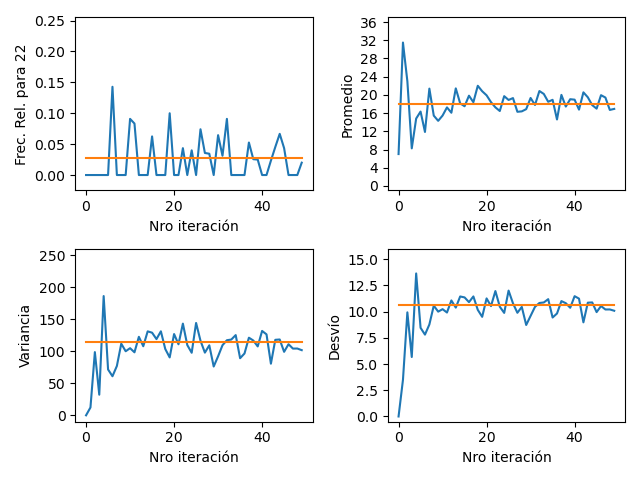
\includegraphics[width=0.75\textwidth]{images/Figure_1.png}
\caption{Simulación de 50 iteraciones.}
\label{fig:50iter}
\end{figure}

\begin{figure}[H]
\centering
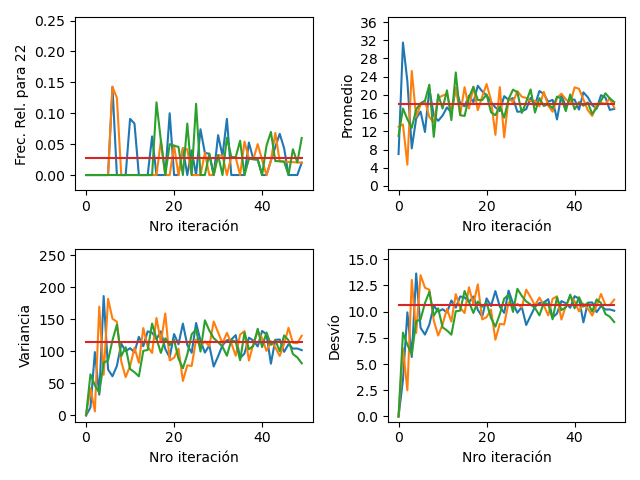
\includegraphics[width=0.75\textwidth]{images/Figure_2.png}
\caption{Comparación de tres simulaciones de 50 iteraciones.}
\label{fig:50iter3}
\end{figure}
 
\begin{figure}[H]
\centering
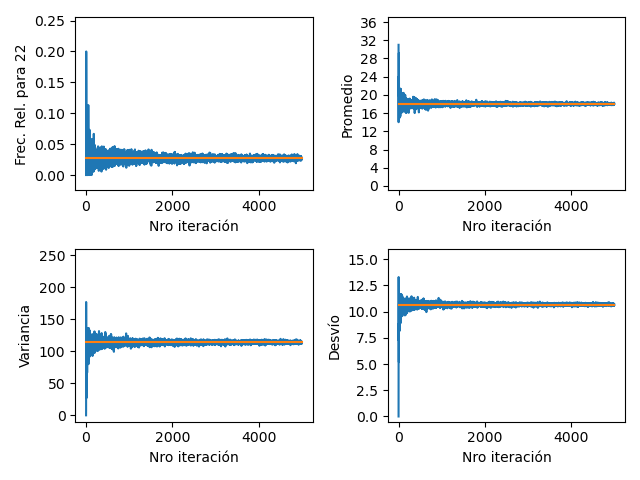
\includegraphics[width=0.75\textwidth]{images/Figure_3.png}
\caption{Simulación de 5000 iteraciones.}
\label{fig:5000iter}
\end{figure}
 
\begin{figure}[H]
\centering
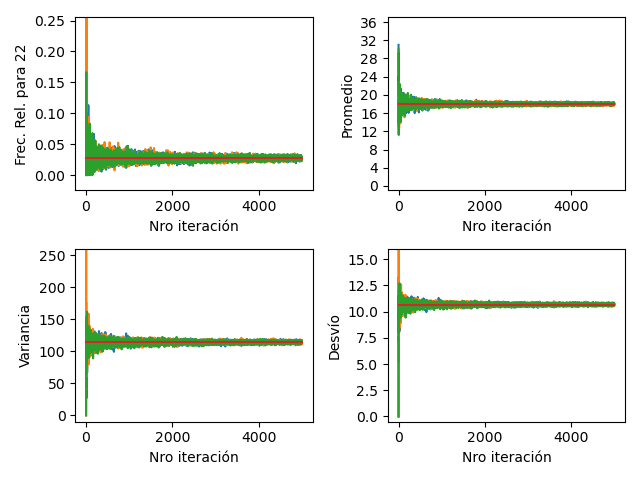
\includegraphics[width=0.75\textwidth]{images/Figure_4.png}
\caption{Comparación de tres simulaciones de 5000 iteraciones.}
\label{fig:5000iter3}
\end{figure}

\end{document}
